% Generated by scripts/generate-paper-figures.ts
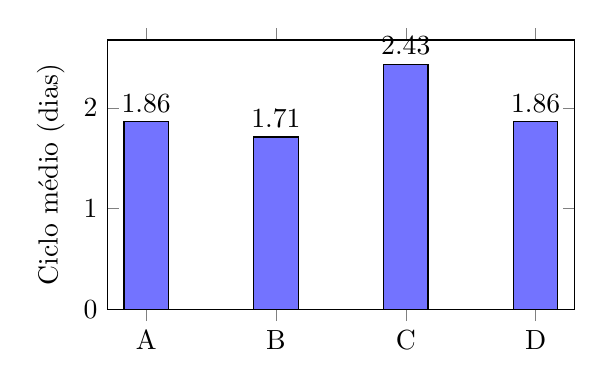
\begin{tikzpicture}
\begin{axis}[
  width=0.62\linewidth,
  height=5cm,
  ybar,
  ymin=0,
  symbolic x coords={A,B,C,D},
  xtick=data,
  xticklabel style={align=center},
  ylabel={Ciclo médio (dias)},
  nodes near coords,
  nodes near coords align={vertical},
  bar width=16pt,
]
\addplot[fill=blue!55] coordinates {(A,1.86) (B,1.71) (C,2.43) (D,1.86)};
\end{axis}
\end{tikzpicture}
